\addcontentsline{toc}{section}{Leaky Container (3)}
\section*{Leaky Container}

\subsection*{Problem}

There is a cup of radius $R$ on the table.
A container that is higher than the cup by $H$
is fully filled with water
and is placed next to the cup in such a way
that the distance between cup's center and its nearest edge is $D$.
Where on the container you should poke a small hole
so there is maximum possible amount of water in the cup
after the water flow stops?

\subsection*{Solution}

We take the cup's top as $0$ of height.
Forget about the finiteness of the container for now.
If the hole is made on height $h$,
than the water should have velocity $v= d \sqrt{g / 2h}$
upon exiting the container to hit distance $d$ (basic kinematics).
To gain velocity $v$
the water level $l$ should be $v^2 / 2 g$ higher than the hole (Bernoulli equation).
So if we poke the hole at $h$,
the water levels that
will hit the nearest and the farthest edges of the cup are
\begin{equation}
    l_{\pm} = h + \frac{(D \pm R)^2}{4h}
\end{equation}
and all the water between $l_-$ and $l_+$ will end up in the cup.
One may notice, that
the difference $l_+ - l_-$ is decreasing on $h$,
and hits infinity at $h=0$.
Here comes the finiteness of the container.

\begin{wrapfigure}{l}{.5\textwidth}
    \centering
    \vspace{-.5cm}
    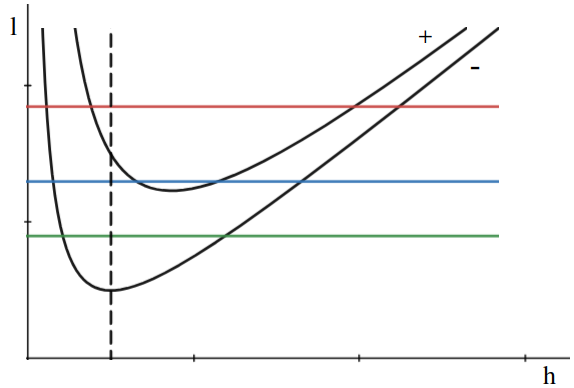
\includegraphics[width = .5\textwidth]{S-1}
    \caption{The water levels,
        at which water will hit the edges of the cup (black solid lines)
        for specific position of the hole (horizontal axis).
        Colorful lines demonstrate different possible values of $H$.
        Dashed black line indicates the minimum of $l_-$.}
    \labelf{S-1}
    \vspace{-.5cm}
\end{wrapfigure}
In order to better understand the situation
let's qualitatively portray $l_\pm$ and $H$ on $h$ \reff{S-1}.
The minima of $l_\pm$ are located at $h_\pm = (D \pm R) / 2$,
and thereby the minimum of $l_-$ is left to that of $l_+$.
We have to choose such $h$,
that the section between $l_+$ and $l_-$ clamped by $H$ is maximal.

If we remember, that the distance without clamping decreases on $h$,
it is easy to verify, that
in case the first intersection of $H$ and $l_+$
is left from the minimum of $l_-$ (the red line case on \reff{S-1}),
that the intersection point itself is the optimal place for a hole.
The intersection point is given by the smaller solution of $H = l_+$
\begin{equation}
    h = \frac{H - \sqrt{H^2 - (D + R)^2}}{2}
\end{equation}
If the intersection is right from $h_-$ (the blue line case)
or there is no intersection at all (the green line case)
then $h$ is just $h_-$.

So the optimal $h$ for the hole is given by
\begin{equation}
    h = \min\inb({\frac{H - \sqrt{H^2 - (D + R)^2}}{2}, \frac{D-R}{2}})
\end{equation}
and when the first argument is undefined we automatically take the second one.

There is also a possibility that no water can end up in the cup.
In that case we are free to make a hole wherever we want.
